%
% File acl2019.tex
%
%% Based on the style files for ACL 2018, NAACL 2018/19, which were
%% Based on the style files for ACL-2015, with some improvements
%%  taken from the NAACL-2016 style
%% Based on the style files for ACL-2014, which were, in turn,
%% based on ACL-2013, ACL-2012, ACL-2011, ACL-2010, ACL-IJCNLP-2009,
%% EACL-2009, IJCNLP-2008...
%% Based on the style files for EACL 2006 by 
%%e.agirre@ehu.es or Sergi.Balari@uab.es
%% and that of ACL 08 by Joakim Nivre and Noah Smith

\documentclass[11pt,a4paper]{article}
\usepackage[hyperref]{acl2019}
\usepackage{times}
\usepackage{graphicx}
\usepackage{latexsym}

\usepackage{url}

\aclfinalcopy % Uncomment this line for the final submission
%\def\aclpaperid{***} %  Enter the acl Paper ID here

%\setlength\titlebox{5cm}
% You can expand the titlebox if you need extra space
% to show all the authors. Please do not make the titlebox
% smaller than 5cm (the original size); we will check this
% in the camera-ready version and ask you to change it back.

\newcommand\BibTeX{B\textsc{ib}\TeX} 

\title{Dataflow Analysis on Rust MIR}

\author{Andres Rios \\
  \texttt{ariossta@andrew.cmu.edu} \\}

\date{}

\begin{document}
\maketitle
\begin{abstract}
    This work presents a tool\footnote{code available at \href{https://github.com/Arios16/dataflow-rs}{https://github.com/Arios16/dataflow-rs}} for performing dataflow analysis on Rust
    programs. It works by leveraging Rust's Mid-level Intermediate
    Representation (MIR), which provides simplified statements and
    control flow. We give an overview of the implementation, describe
    the API and show an example of the tool in practice.
\end{abstract}

\section{Introduction}

Dataflow analysis is a powerful tool used in optimizers and static analysis
tools to reason about programs. Tools like Soot \cite{Soot} enable users
to, among other things, perform dataflow analysis in Java programs, and similar tools
exist for other languages. However, no such tool exists (to this author's knowledge) 
that enables a user to easily perform data flow analysis on Rust programs without 
having to implement the underlying algorithms themselves. \\

This work implements a dataflow analysis tool on top of Rust's MIR 
so that a user only needs to specify a lattice and flow functions to be
able to perform dataflow analysis on Rust programs.

\section{Related Work}

The algorithm implemented in this work is Kildall's algorithm
\cite{Kildall:1973:UAG:512927.512945}.
It works by mantaining a worklist of program nodes yet to be analyzed
(initialized with the entry node of the program) and a mapping from
nodes to dataflow information on node entry.
On each iteration, a node is taken off the worklist, the entry dataflow 
information is modified based on the node's statement(s), and then that information
is propagated to the input of the node's successors, as specified by the
CFG of the program. The nodes which have  their input modified
are then added to the worklist.\\

The MIR was originally proposed in Rust's RFC 1211 \cite{MIR}. The
MIR (short for Mid-level Intermediate Representation) is a simplified representation
of a Rust program. Each function is represented as a set of basic blocks, where
each basic block consists of a sequence of statements and a terminator. The statements
we are interested in are assignment statements, where an lvalue is assigned to an rvalue.
Rvalues cannot be arbitrarily complex expressions - they are at most the result of a
binary operator. Terminators are how the control flow is represented. There are
several types of terminators (goto, switch, function calls, etc.). An example of a Rust program
and its simplified MIR is shown in figure \ref{mir}.


\begin{figure}[h]
    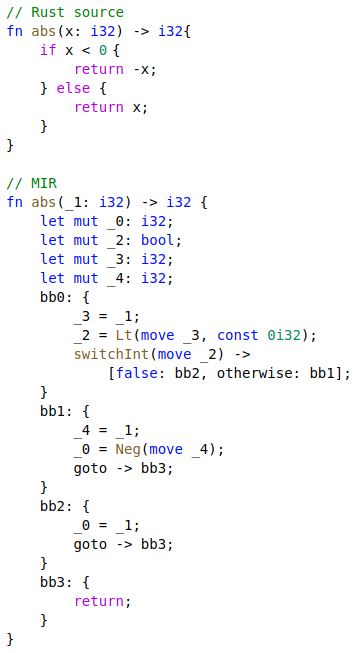
\includegraphics[width=7.6cm]{img/mir.png}
    \caption{Example of a function and its (simplified) MIR counterpart}
    \label{mir}
\end{figure}


\section{Implementation Overview}

\subsection{Internal Details}

The analysis itself is implemented as a compiler callback. After the MIR is
generated, compiling is stopped and the analysis is performed.\\

The CFG nodes on which the analysis operates are the MIR's basic blocks, 
not statements. This is not leaked to the public; users need only propagate
information through individual statements. Analysing whole basic blocks at
a time enables us to keep track of which variables are equal to others, so 
that the collected dataflow information can be more precise. The reason this is useful
is because the MIR always assigns variables to a temporary before using them
in a conditional expression. Any information we gain about the temporary from 
the result of the conditional is also gained about the actual variable, but for
that we need to be able to reason that both variables are equal when the 
conditional is executed. Temporaries are not assigned more than once per basic block,
so reasoning about them is easier within a basic block. \\

As figure \ref{mir} shows, \texttt{switch} statements do not directly operate on an rvalue
producing a boolean, but rather, assign the boolean to a variable and then switch on
that variable. This makes it harder to propagate conditional information. A common pattern
is for the boolean to be produced within the same basic block (as is the case in figure \ref{mir}), followed by a possible \texttt{Not}
statement. The analysis can correctly propagate conditional information in such cases. However,
in some cases the boolean value inside the \texttt{switch} statement can be generated from multiple
places (e.g. multiple blocks assign a boolean to a variable and then use a \texttt{goto} to jump
to a block that does a \texttt{switch} on that variable). In that case, it is difficult to determine
which information must be propagated depending on the result of the \texttt{switch}, as the condition
being evaluated could be one of many. In this case, the current implementation loses the opportunity to refine the dataflow
information in the \texttt{switch}, simply treating it as a \texttt{goto} with multiple destinations. This is sound,
but not as precise as it could be.

\subsection{Public API}

The most important part of the public API is the \texttt{Lattice} trait,
shown in figure \ref{fig:lattice}. Traits are similar to interfaces in
other languages, specifying a set of functions that functions have to
implement to satisfy the trait. The lattice trait requires the type
implementing it to be able to specify the top and bottom elements, how
to join two lattice elements, and how to flow information through
assignments and branches. It also demands a method to deal with function
calls, but interprocedural analysis is not yet supported. This method
exists purely so that the lattice can assign a top element to the
appropriate variable, if necessary.\\

Though lattices can take any form, a very common pattern is to have a lattice
that maps local variables to a simpler lattice, as is the case with the canonical
sign analysis or interval analysis. For this use case, the API offers the
\texttt{SimpleLattice} trait, shown in figure \ref{fig:simple_lattice}.
Once \texttt{SimpleLattice} is implemented for a type \texttt{T}, \texttt{Lattice}
is automatically implemented for a hashmap mapping local variables to \texttt{T}
values. This eases the burden of implementation for users with this simpler
use case.\\

The last piece of the public API is the \texttt{run} function, which receives two arguments:
a string \texttt{target}, specifying the path to the Rust source file on which to run the
analysis, and a function \texttt{F} that takes a statement and a lattice element as input.
The function \texttt{F} will then be called for every statement in the MIR along with the
dataflow information that was gathered about that statement. The user can use this \texttt{F} function
to report errors or for other purposes.


\begin{figure}
    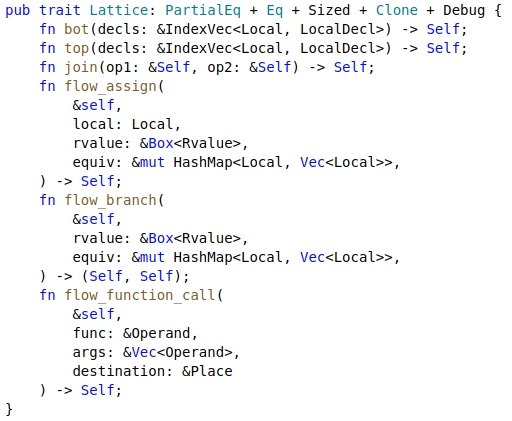
\includegraphics[width=7.6cm]{img/lattice.png}
    \caption{\texttt{Lattice} trait}
    \label{fig:lattice}
\end{figure}

\begin{figure}
    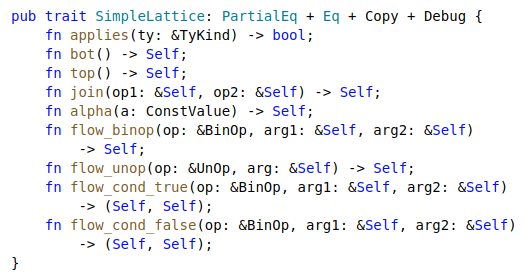
\includegraphics[width=7.6cm]{img/simplelattice.png}
    \caption{\texttt{SimpleLattice} trait}
    \label{fig:simple_lattice}
\end{figure}

\section{Example: Sign Analysis}

An example using this tool to perform sign analysis can be found with the
linked code. The example uses the \texttt{SimpleLattice} API.\\

The simple lattice definition can be found in figure \ref{fig:sign_lattice}. The different
variants of the \texttt{enum} represent whether the variable is zero, lower than zero, greater than zero, etc.
The \texttt{SimpleLattice} trait is implemented for this type.
As mentioned before, this gains us an implementation of \texttt{Lattice}
for the type \texttt{HashMap<Local, PreciseSign>}. The analysis is then run
using this lattice along with a function that reports an error if a variable
that may be negative is cast as an unsigned integer (which causes an underflow).\\

\begin{figure}
    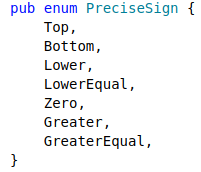
\includegraphics[width=4cm]{img/precise_sign_analysis.png}
    \caption{\texttt{PreciseSign} simple lattice definition}
    \label{fig:sign_lattice}
\end{figure}

\begin{figure}
    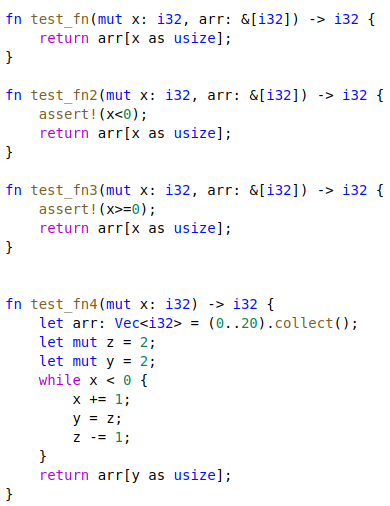
\includegraphics[width=7.6cm]{img/test_functions.png}
    \caption{Functions being analyzed}
    \label{fig:test_functions}

    \vspace{1cm}

    \begin{verbatim}
Analysing function: "test_fn"
Possible error at example.rs:3:16: 
3:26. Value being cast as unsigned 
integer may be lower than 0.

Analysing function: "test_fn2"
Error at example.rs:8:16: 8:26. 
Value lower than 0 is being cast 
as unsigned integer.

Analysing function: "test_fn3"

Analysing function: "test_fn4"
Possible error at example.rs:26:16: 
26:26. Value being cast as unsigned 
integer may be lower than 0.
    \end{verbatim}
    \caption{Output of the analysis}
    \label{fig:analysis_output}
\end{figure}


The functions being analyzed can be found in figure \ref{fig:test_functions}, while
the output of the analysis can be found in figure \ref{fig:analysis_output}.\\

In the first example, \texttt{x} may be anything, and so it may be lower than 0
when it is cast as \texttt{usize}. This is reported by the analysis.\\

In the second example, the \texttt{assert} statement makes sure that if the program
execution reaches the cast, then \texttt{x} is guaranteed to be negative, and so
the analysis reports a definite error.\\

In the third example, the \texttt{assert} statement ensures that \texttt{x} is non-negative
if the cast is reached. Thus, the analysis finds no errors.\\

The last example is slightly more complex. Initially, \texttt{y} (the variable that is later cast as \texttt{usize})
is positive, and it remains positive for the first iterations of the loop. However, if we iterate enough times
then it may become negative. Because the number of iterations is unknown (it depends on the parameter \texttt{x}),
then we may or may not have an error. The analysis understands this control flow construct, and so reports
that there is a possible error.


\section{Conclusion and Future Work}

A working dataflow analysis tool is presented that can be used to relatively
easily perform analysis on Rust programs. However, there are some limitations 
on this work:

\begin{itemize}
    \item The analysis is strictly intra-procedural. Implementing iter-procedural analysis
    is left as future work.
    \item The analysis can't propagate path-sensitive information for \texttt{if} statements
    with complex conditionals. This is due to the difficulties described in section 3.1.
    Future research is required to determine how to correctly propagate path-sensitive information
    in these cases.
\end{itemize}

\bibliography{acl2019}
\bibliographystyle{acl_natbib}

\end{document}
